\documentclass[10pt]{article}
\usepackage[paperwidth=40in, paperheight=40in]{geometry}
\usepackage[usenames]{color} %used for font color
\usepackage{amssymb} %maths
\usepackage{amsmath} %maths
\usepackage[utf8]{inputenc} %useful to type directly diacritic characters

%%% Sans serif text font
\usepackage[scaled]{helvet}
\renewcommand*\familydefault{\sfdefault}\usepackage[T1]{fontenc}
%%%

\usepackage{skull}
\usepackage{tikz}
\usetikzlibrary{positioning}
\usetikzlibrary{arrows}
\usetikzlibrary{fit}
\usetikzlibrary{calc}
\usetikzlibrary{automata}
\usetikzlibrary{decorations.markings}
\usetikzlibrary{decorations.pathreplacing}

\tikzset{>=latex}
\tikzstyle{snode}=[black,draw=black,line width=1.5pt,shape=circle,fill=white,minimum size=8mm]
\tikzstyle{obnode}=[black,draw=black,line width=1.5pt,shape=circle,fill=black!20!white,minimum size=8mm]
\tikzstyle{detnode}=[black,draw=black,line width=1.5pt,densely dotted,shape=circle,fill=white,minimum size=8mm]
\tikzstyle{constnode}=[black,draw=black,line width=1.5pt,shape=rectangle,fill=white,minimum size=8mm]
\tikzstyle{mincnode}=[black,draw=black,line width=0.75pt,shape=rectangle,fill=white,minimum size=3mm]
\tikzstyle{blnode}=[white,draw=black,line width=1pt,shape=circle,fill=black,minimum size=1mm,font=\scriptsize,inner sep=1pt]
\tikzstyle{ylnode}=[black,draw=black,line width=1pt,shape=circle,fill=yellow,minimum size=1mm,font=\scriptsize,inner sep=1pt]
\tikzstyle{taro}=[->,line width=2pt,color=black]
\tikzstyle{thintaro}=[->,line width=0.75pt,color=black]
\tikzstyle{dtaro}=[->,line width=2pt, densely dotted,color=black]
\tikzstyle{smod}=[black, draw=black, line width=2pt, fill=white, shape=rectangle, rounded corners, minimum size=10mm, minimum width=20mm]
\tikzstyle{obmod}=[black, draw=black, line width=2pt, fill=black!20!white, shape=rectangle, rounded corners, minimum size=10mm, minimum width=20mm, minimum width=20mm]

\definecolor{shc}{RGB}{238,224,229}
\definecolor{shc2}{RGB}{182,152,195}
\definecolor{brnt}{RGB}{221,132,13}

\begin{document}
\[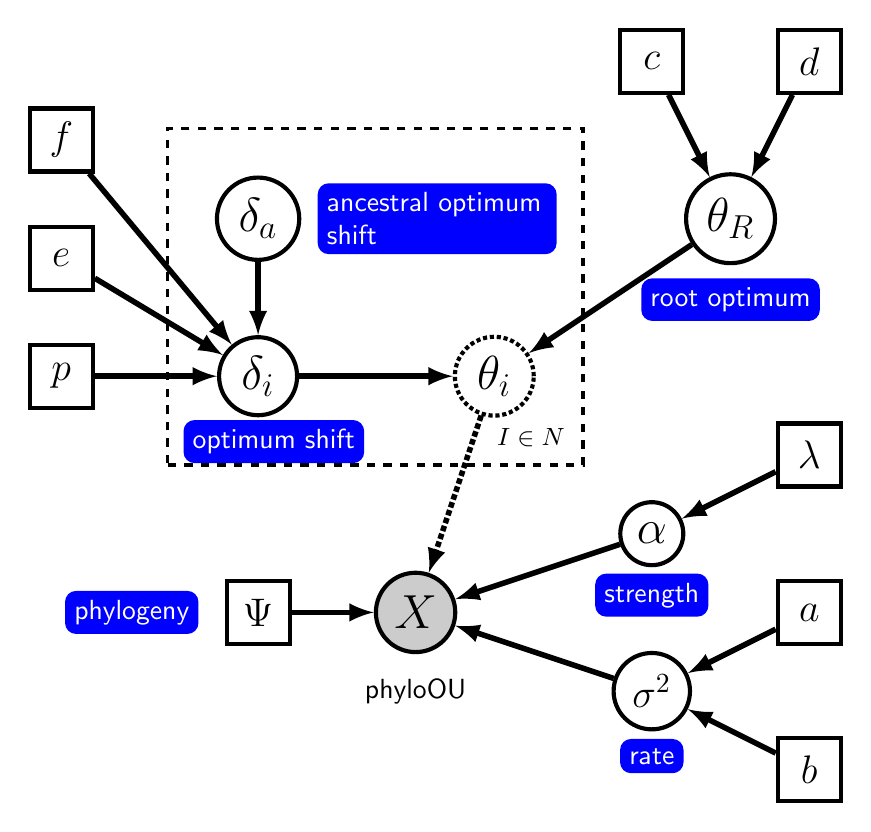
\begin{tikzpicture}
\node[obnode] (nx) at (1,1) {\LARGE $X$};
\node[detnode] (thetai) at ($(nx)+(1,3)$) {\LARGE $\theta_i$};
\node[snode] (rmi)  at ($(thetai)+(-3,0)$) {\LARGE $\delta_i$};
\node[constnode] (p) at ($(rmi)+(-2.5,0)$) {\Large $p$};
\node[constnode] (s) at ($(rmi)+(-2.5,1.5)$) {\Large $e$};
\node[constnode] (m) at ($(rmi)+(-2.5,3)$) {\Large $f$};
\node[snode] (rma)  at ($(rmi)+(0,2)$) {\LARGE $\delta_a$};
\node[constnode] (phylo) at ($(nx)+(-2,0)$) {\Large $\Psi$};
\node[snode] (sigma2r) at ($(thetai)+(3,2)$) {\LARGE $\theta_R$};
\node[constnode] (l) at ($(sigma2r)+(-1,2)$) {\Large $c$};
\node[constnode] (u) at ($(sigma2r)+(1,2)$) {\Large $d$};
\node[snode] (alpha)  at ($(nx)+(3,1)$) {\LARGE $\alpha$};
\node[snode] (sigma2)  at ($(nx)+(3,-1)$) {\Large $\sigma^2$};
\node[constnode] (lambda)  at ($(alpha)+(2,1)$) {\Large $\lambda$};
\node[constnode] (a)  at ($(sigma2)+(2,1)$) {\Large $a$};
\node[constnode] (b)  at ($(sigma2)+(2,-1)$) {\Large $b$};
\draw [taro] (rmi) -- (thetai);
\draw [taro] (sigma2r) -- (thetai);
\draw [taro] (rma) -- (rmi);
\draw [taro] (phylo) -- (nx);
\draw [taro] (p) -- (rmi);
\draw [taro] (m) -- (rmi);
\draw [taro] (s) -- (rmi);
\draw [dtaro] (thetai) -- (nx);
\draw [taro] (l) -- (sigma2r);
\draw [taro] (u) -- (sigma2r);
\draw [taro] (alpha) -- (nx);
\draw [taro] (sigma2) -- (nx);
\draw [taro] (a) -- (sigma2);
\draw [taro] (b) -- (sigma2);
\draw [taro] (lambda) -- (alpha);
\node at ($(nx)+(0,-1)$) {phyloOU};
\node[white, fill=blue, shape=rectangle, rounded corners] at ($(phylo)+(-0.75,0)$) [left]{phylogeny};
\node[white, fill=blue, shape=rectangle, rounded corners] at ($(sigma2r)+(0,-0.75)$) [below]{root optimum};
\node[white, fill=blue, shape=rectangle, rounded corners] at ($(rmi)+(0.2,-0.55)$) [below]{optimum shift};
\node[white, fill=blue, shape=rectangle, rounded corners] at ($(alpha)+(0,-0.5)$) [below]{strength};
\node[white, fill=blue, shape=rectangle, rounded corners] at ($(sigma2)+(0,-0.6)$) [below]{rate};
\node[white, fill=blue, shape=rectangle, rounded corners, text width=2.8cm] at ($(rma)+(0.75,0)$) [right]{ancestral optimum shift};
% \node[white, fill=blue, shape=rectangle, rounded corners] at ($(sigma2)+(0.75,0)$) [right]{rate};
\node[rectangle,dashed, very thick, inner sep=6mm, draw=black!100, fit = (thetai)(rmi)(rma)] (rateplate) {};
\node[anchor=south east,inner sep=7pt] at (rateplate.south east) {\small $I \in N$};
\end{tikzpicture}
\]
\end{document}